\subsection{Slow dynamics}

\begin{frame}{Modelling of Water Distribution Network}{Slow dynamics}
	\begin{columns}
		\begin{column}{.5\textwidth}
			\begin{itemize}
				\item Fundamentals
				\begin{equation*}
					p \propto h 
				\end{equation*}
				\begin{equation*}
					\dot{V} = q
				\end{equation*}
				\item Assume constant cross sectional area A
				\begin{equation*}
					V \propto h \implies V \propto p 
				\end{equation*}
				\begin{equation*}
					\dot{p} \propto \dot{V} \wedge \dot{V} = q \implies \dot{p} \propto q
				\end{equation*}
				\item We arrive at
				\begin{equation*}
					\dot{p} = -\tau q \text{,  where}
				\end{equation*}	
				\begin{equation*}
					\tau = \rho g \frac{1}{A}
				\end{equation*}	
			\end{itemize}
		\end{column}
		\begin{column}{.5\textwidth}\raggedleft
			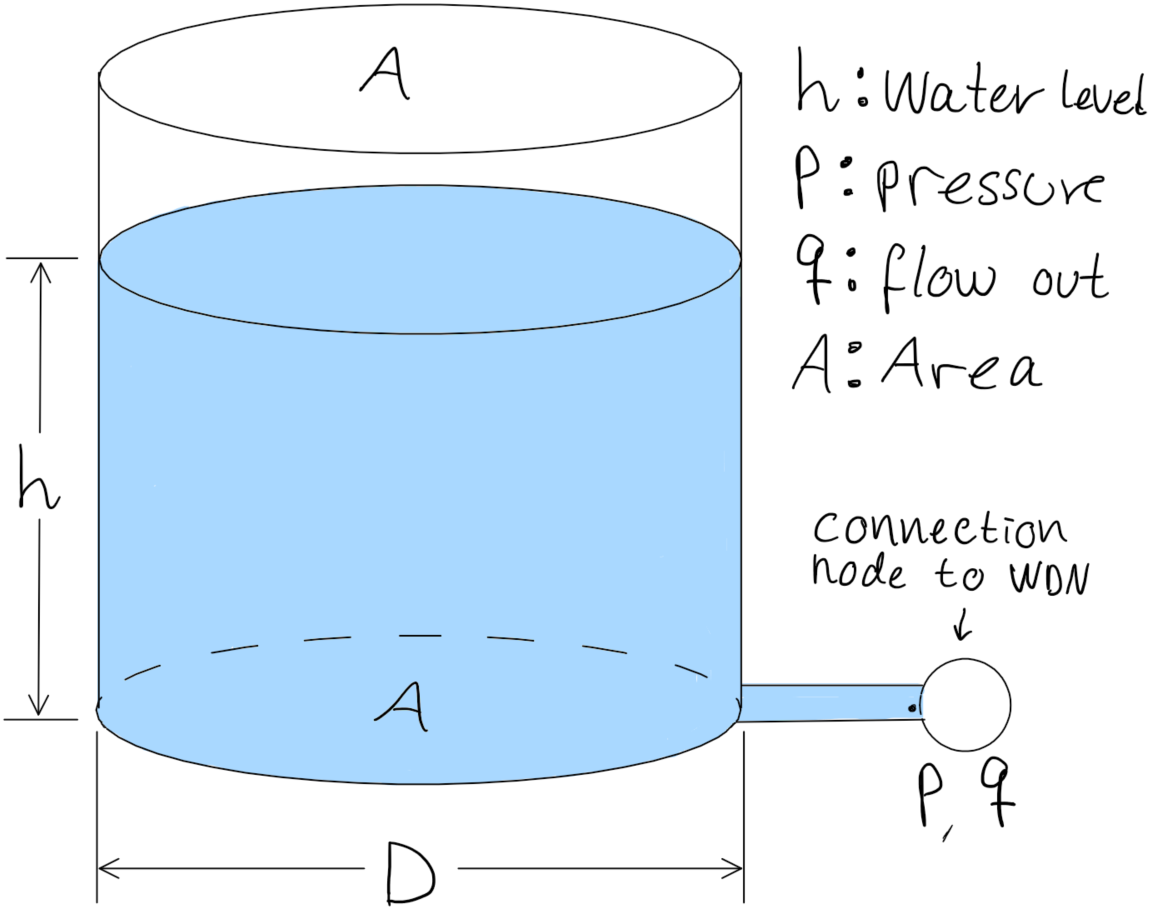
\includegraphics[width=1\linewidth]{Topics/SlowDynamicsLinearisation/Graphics/Tank_sketch.png}
		\end{column}
	\end{columns}
\end{frame}

\begin{frame}{Modelling of Water Distribution Network}{State space formulation of slow dynamics}
	\begin{figure}[h!]
		\centering
		\resizebox{\columnwidth}{!}{
				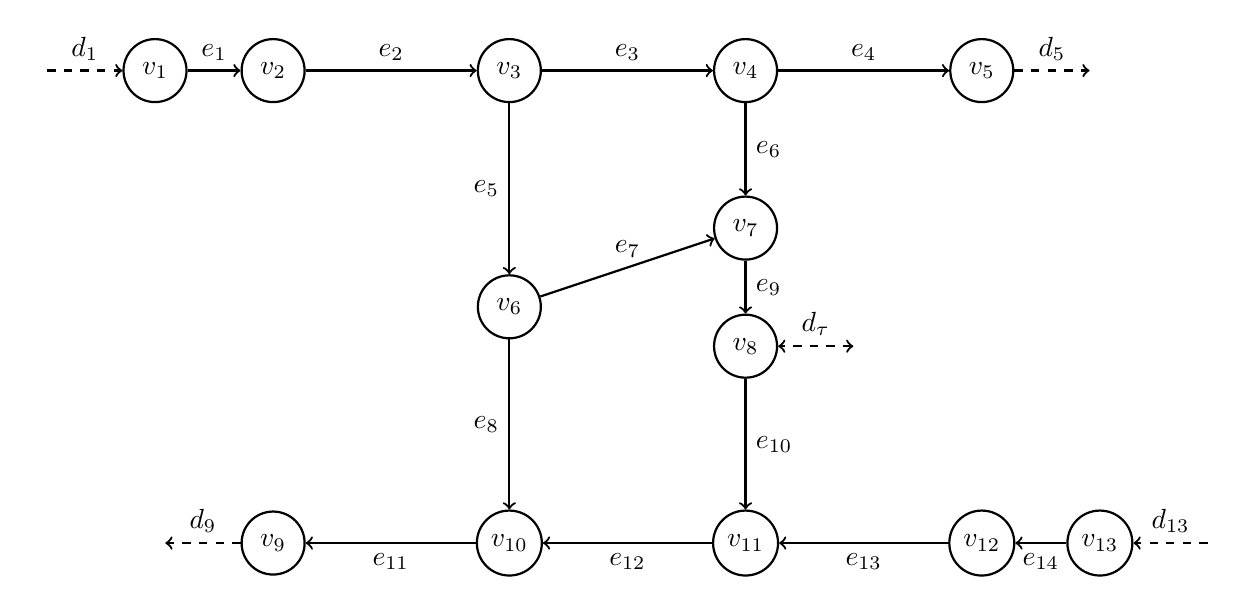
\begin{tikzpicture}[node distance=30mm, thick, main/.style = {draw,circle,minimum size=0.8cm}] 
		\node (1)  {};
		\node[main] (2) [node distance={15mm},right of=1] {$v_1$}; 
		\node[main] (3) [node distance={1.5cm},right of=2] {$v_2$};
		\node[main] (4) [right of=3] {$v_3$};
		\node[main] (5) [right of=4] {$v_4$};
		\node[main] (6) [right of=5] {$v_5$};
		\node (7) [node distance={15mm},right of=6] {};
		%Create 3 (4) nodes in middle part of graph
		\node[main] (8) [below of=4] {$ v_6 $};
		\node[main] (9) [node distance={20mm},below of=5] {$ v_7 $};
		\node[main] (11) [node distance={15mm},below of=9] {$ v_8 $};
		\node (10) [node distance={15mm},right of=11] {};
		%First 5 (7) nodes in bottom part of graph
		\node[main] (12) [below of=8] {$ v_{10} $};
		\node[main] (13) [left of=12] {$ v_9 $};
		\node(14) [node distance={15mm},left of=13] {};
		\node[main] (15) [right of=12] {$ v_{11} $};
		\node[main] (16) [right of=15] {$ v_{12} $};
		\node[main] (17) [node distance={1.5cm},right of=16] {$ v_{13} $};
		\node(18) [node distance={15mm},right of=17] {};
		
		%Edges with direction
		\path [->] (2) edge node[above] {$e_{1}$} (3); 	%Edge v1 -> v2
		\path [->] (3) edge node[above] {$e_{2}$} (4); 	%Edge v2 -> v3
		\path [->] (4) edge node[above] {$e_{3}$} (5); 	%Edge v3 -> v4
		\path [->] (5) edge node[above] {$e_{4}$} (6); 	%Edge v4 -> v5
		
		\path [->] (4) edge node[left] {$e_{5}$} (8); 	%Edge v3 -> v6
		\path [->] (5) edge node[right] {$e_{6}$} (9); 	%Edge v4 -> v7
		\path [->] (8) edge node[above] {$e_{7}$} (9); 	%Edge v6 -> v7
		\path [->] (8) edge node[left] {$e_{8}$} (12); 	%Edge v6 -> v10
		\path [->] (9) edge node[right] {$e_{9}$} (11); 	%Edge v7 -> v8
		\path [->] (11) edge node[right] {$e_{10}$} (15);	 %Edge v8 -> v11
		
		
		\path [->] (12) edge node[below] {$e_{11}$} (13); %Edge v10 -> v9
		\path [->] (15) edge node[below] {$e_{12}$} (12); %Edge v11 -> v10
		\path [->] (16) edge node[below] {$e_{13}$} (15); %Edge v12 -> v11
		\path [->] (17) edge node[below] {$e_{14}$} (16); %Edge v13 -> v12
		
		%External flows
		\draw[->,dashed,] (1) -- node[above] {$d_1$} (2); %Create d1
		\draw[->,dashed,] (6) -- node[above] {$d_5$} (7); %Create d5
		\draw[->,dashed,] (13) -- node[above] {$d_9$} (14); %Create d13
		\draw[->,dashed,] (18) -- node[above] {$d_{13}$} (17); %Create d13
		\draw[<->,dashed,] (10) -- node[above] {$d_\tau$} (11); %Create d_tau
	\end{tikzpicture} }
		\label{fig:tikzWDNGraph}
	\end{figure}  
	In context of WDN we now consider flows to and from network as external demands $ d_i $
\end{frame}

\begin{frame}{Modelling of Water Distribution Network}{State space formulation of slow dynamics}
	Mass conservation holds, and such
	\begin{equation*}
		d_n = -\sum_{i=1}^{n-1}d_i \implies d_\tau = - (d_p + d_c)
	\end{equation*}
	\begin{equation*}
		\dot{p} = -\tau d_\tau = \tau (d_p + d_c)
	\end{equation*}	
	When discretised by forward Euler:
	\begin{equation*}
		p_\tau(k+1) = p_\tau(k) - \tau d_\tau(k) t_s = p_\tau(k) + \tau(d_p(k) + d_c(k)) t_s
	\end{equation*}
	Which corresponds to a discrete, linear state-space model:
	\begin{equation}
		p_\tau(k+1) = Ap_\tau(k) + B_pd_p(k) + B_cd_c(k)
	\end{equation}
	\begin{equation*}
		d_p = \begin{bmatrix}
			d_1 \\ d_{13}
		\end{bmatrix},
		d_c = \begin{bmatrix}
			d_5 \\ d_9
		\end{bmatrix},
		B_p = B_c = t_s  \begin{bmatrix}
			\tau & \tau
		\end{bmatrix},
		A = 1
	\end{equation*}
\end{frame}


\subsection{Linearisation}
\begin{frame}{Modelling of Water Distribution Networks}{Linearisation}
	Fast dynamics are non linear - linearisation is needed.\\
	In near vicinity of linearisation point $ x_0 $,
	\begin{equation*}
		\dot{x} \approx f(x_0) + \nabla f\bigg\rvert_{x_0} (x-x_0)
	\end{equation*}
	Recalling the fast dynamics differential equation is given as
	\begin{equation}\label{eq:NonLinearModelSimplified}
		\begin{split}
			\dot{q}_n &=  -\mathcal{P}\Phi\Big(\lambda(q_n)+\mu(q_n,\Theta)+\alpha(q_n,\omega)\Big) +\\ &\mathcal{P}\Big(\Psi(\bar{h}-\mathbf{1}h_0) + \mathcal{I}(p_{\tau}-\mathbf{1}p_0)\Big) \\
		\end{split}	
	\end{equation}
	The linear model such becomes
	\begin{equation}\label{eq:SymbolicLinearisation}
		\begin{split}
			\dot{q}_n &\approx f(x_0) + \frac{\partial f}{\partial q_n}\bigg\rvert_{x_0} \tilde{q}_n + \frac{\partial f}{\partial \Theta}\bigg\rvert_{x_0} \tilde{\Theta} + \frac{\partial f}{\partial \omega}\bigg\rvert_{x_0} \tilde{\omega} +  \frac{\partial f}{\partial p_\tau}\bigg\rvert_{x_0} \tilde{p}_\tau
			\\
		\end{split}
	\end{equation}
	where $x_0 = \{q_0,\Theta_0,\omega_0, p_{\tau_0} \}$, $ \tilde{q} =q-q_0$, likewise for $ \tilde{\Theta} $, $ \tilde{\omega}$, $\tilde{p_{\tau}}  $
\end{frame}

\begin{frame}{Modelling of Water Distribution Networks}{Linearisation}
	The full linearised model is then obtained as
	\begin{equation}\label{eq:SymbolicLinearisationExpanded}
		\begin{split}
			\dot{q}_n \approx f(x_0) -\mathcal{P}\Phi & \Bigg(a_1\omega_0 + \Big(|q_0|+\text{sign}(q_0)q_0\Big)\\
			& \Bigg(K_\lambda + a_2 + \frac{1}{(K_v \Theta_0)^2}\Bigg) \tilde{q}_n \Bigg)  \\
			- \mathcal{P}\Phi&\Bigg(\Big(-|q_0|q_0 \frac{2}{K_v^2 \Theta_0^3}\Big) \tilde{\Theta}\Bigg) \\
			- \mathcal{P}\Phi&\Bigg(\Big(a_1 q_0 + 2a_0\omega_0\Big) \tilde{\omega}\Bigg) \\
			+ \mathcal{P} \mathcal{I}& \tilde{p}_\tau
		\end{split}
	\end{equation}
The equation can be simplified further making some assumptions
\end{frame}

\begin{frame}{Modelling of Water Distribution Networks}{Linearisation}
	Equilibrium disappears, valve and tank dynamics assumed to be constant disturbances 
	\begin{equation}\label{eq:SymbolicLinearisationSimplified}
		\begin{split}
			\dot{q}_n \approx -\mathcal{P}\Phi &\Bigg(a_1\omega_0 + \Big(|q_0|+\text{sign}(q_0)q_0\Big) \\
			&\Bigg(K_\lambda + a_2 + \frac{1}{(K_v \Theta_0)^2}\Bigg) \tilde{q}_n \Bigg) \\
			- \mathcal{P}\Phi&\Bigg(\Big(a_1 q_0 + 2a_0\omega_0\Big) \tilde{\omega}\Bigg)
		\end{split}
	\end{equation}
	
\end{frame}
